\documentclass{article}
\usepackage[utf8]{inputenc}
%\usepackage{appendix}
\usepackage{graphicx}
\graphicspath{{./images/}}
\usepackage{float}
\usepackage{mwe}
\usepackage{hyperref}
\usepackage{xurl}

%margins
\usepackage{geometry}
 \geometry{
%  letter,
 left=1in,
 top=1in,
 right=1in,
 bottom=1in
}
 
\title{How to Move from Windows to Linux}
%\subtitle{ENGL-321}
\author{Steven Glasford}
\date{\today}

\begin{document}

\maketitle

\tableofcontents

\section{Introduction}
There are many different types of operating systems globally. Most people know the basic ones like Windows, Mac, Android, iOS, and maybe some remember Blackberry. Every computer or smart device uses an operating system, but they are not all the same. Windows, macOS, iOS are all proprietary. Proprietary software means that a person must pay to use their services and makes it hard, if not impossible, to see what the operating system is doing. 


Proprietary software can very often be filled with bugs and is vulnerable to becoming out of date. However, proprietary software is often very desirable, and most of the world's essential software like iPhones, Windows, Photoshop, and Fortnight use this software model. Most of the world, however, does not use this type of software. Most of the world runs on what is known as Free and Open Source Software (FOSS). FOSS allows anyone to alter the software for their liking, beyond installing new applications or anything else. Alteration makes it highly desirable for large companies who wish to make money from altering open-source software to make a product. Sometimes FOSS is the basis for the software that people use. A good example of altering a FOSS program is MacOS, based on UNIX. Unix no longer exists and in its place is Linux. This alteration is why both Linux and macOS have remarkably similar terminal interfaces.


For almost every example of proprietary software, there is an open-source alternative. Android is open source, although Android's license allows companies to alter the android operating system, which sometimes makes it proprietary again. Again this new proprietary software also leads to security vulnerabilities when the phone no longer receives updates. 


Sometimes open source software is the only option for an application. One of the newest and most compelling examples is Bitcoin. Anyone can inspect the Bitcoin application and blockchain. Anyone can change bitcoin and modify it to make a new cryptocurrency, which has happened many times. Ethereum is a modified version of Bitcoin with many new features. Monero is a variant of bitcoin that has beefed up security. Another example is AES, which is an encryption scheme used to protect WiFi networks and secure connections to websites like Facebook and Google.
\\
According to ZDNet, about 78\% of businesses use open-source software in some capacity (see page \pageref{78percent} section \ref{sources} part \ref{78percent}) with about 3\% not using it at all. And of the websites that people use, about 96\% use Linux as their operating system (see page \pageref{WWWrunsOnLinux} in section \ref{sources} part \ref{WWWrunsOnLinux}). This high usage is due to Linux's status as an open-source project, its fantastic ability to be customized, as well as its military strength security. Linux is ubiquitous worldwide, and in this instruction, we will learn how to add it to your life.

\section{Requirements}
\subsection{Supplies needed}
In this tutorial, we will need the following:
\begin{itemize}
    \item A computer we want Linux on that has Windows on it already.
    \item An unused flash drive.
\end{itemize}

\subsection{Warnings}
\begin{itemize}
    \item Following these instructions will wipe all data from the computer you are trying to put Linux on and wipe all data from the flash drive.
    \item Make sure all data your data, as this will wipe both your computer and your flash drive.
    \item DATA RECOVERY IS EXTREMELY DIFFICULT AND EXPENSIVE IF YOU DO NOT BACKUP.
    \item Do this on devices that are not your primary devices if possible.
\end{itemize}

\section{Installation}
Linux is very complicated and has many different parts. The following sections will make it easier to follow and understand.

\subsection{Linux Variants and Manjaro}
In this document, we will be moving from Windows, which is proprietary, to a version of Linux called Manjaro, based on Arch Linux, which uses a "Rolling release." A rolling release allows a person always to have the most up-to-date software available, and immediately when an update is available, the computer will be able to update to this version. A rolling release provides many advantages from the alternative known as "staggered releases." Ubuntu and Debian Linux use staggered releases. Rolling releases have some problems. Most notably, they have "bleeding edge" updates; these are updates that have not undergone rigorous testing. Untested updates can, at times, make the computer unstable and even crash. Manjaro fixes this problem by only rolling into a new update once the update is marked as stable by the developers. This method of stability allows for Manjaro to be very stable. It allows for the vast amount of software that can be installed on Arch Linux also to be able to be installed on Manjaro.  


Manjaro is also very easy to use and install onto a new computer, which is exceptionally complicated on Arch Linux. Arch provides a tremendous amount of customization, which adds to its highly advanced nature. 

I will be using Manjaro Linux XFCE in this instruction. However, many others exist like Ubuntu, Debian, Mint, Gentoo, OpenSUSE, Tails, OpenBSD, Elementary, Fedora, and hundreds more. There are also many different types of desktop displays for Linux, with Gnome, XFCE, Plasma being the largest and most supported, but others like Deepin DDE, Cinnamon, Mate, and hundreds of others. The website DistroWatch.com is beneficial and provides many resources to find your perfect type of Linux. The link for DistroWatch is \url{https://distrowatch.com/}. These instructions will be using Manjaro XFCE as it is my favorite type of Linux.


\subsection{Image Files and your Flash Drive}\label{imageFile}
Whatever the type of Linux you choose, you must get an image file. Image files are huge files that will be written on your flash drive. The following will walk through getting the image file and putting the image onto the flash drive.

\begin{enumerate}
    \item Please go to the website \url{https://manjaro.org/downloads/official/xfce/} and download the file the ISO file (This is the Image File, and will take a while as it is a huge file). See figure \ref{fig:downloadPage} for help.
    \item Next, we need to put the image file onto the flash drive. Please go to \url{https://rufus.ie/} and download Rufus 
    \begin{enumerate}
        \item After Downloading, run the program called Rufus. 
        \item Windows might ask if you want to install Rufus like in figure \ref{fig:runRufus}, say yes, Rufus is a safe piece of software.
        \item If asked to choose whether you want Rufus to check for updates as in figure \ref{fig:updateRufus}, check yes if you care, no if you do not care. 
    \end{enumerate} 
    \item After installing Rufus, open the program, and insert your blank or unused flash drive into the computer. 
    \item For the "Boot Selection" option, find and select the location of the image file that you downloaded earlier.
    \item\label{rufusEnd} A regular person will not need to alter any other parts of Rufus, and the "START" button at the bottom of the page should be blue-ish. Click this button. It may warn you that you are ready to wipe the flash drive and agree to this if prompted.
    \item Take a break, as this part will take a while. Rufus will be complete once the "READY" bar at the bottom of the screen is entirely Green (see figure \ref{fig:rufusDone}).
    \item After Rufus is complete, shut down your computer and get ready to install Linux on your machine and continue to section \ref{liveboot}.
\end{enumerate}


\subsection{Live Booting and Trying Linux}\label{liveboot}
After getting the ISO on the computer, you must first boot into the flash drive. The process of booting into a flash drive is unique to your particular computer, and I cannot make a general statement about how to do it. Nevertheless, it would be best to boot from a flash drive on your computer if you found out how to boot. For me booting from the flash drive is very easy. When I boot up, it will ask me which device I want to boot into, so I choose the flash drive I put the ISO image on (see figure \ref{fig:bootIntoFlash}. The flash drive is usually descriptive and typically is the manufacture of the flash drive. 
\begin{enumerate}
    \item Boot into the flash drive, this is dependent on your computer, and additional research should be done to figure out how to do this.
    \item When first booting, there will be a flash of text on the screen as seen in figure \ref{fig:bootSequence}, this is normal, and Linux will boot shortly.
    \item Once booted, it will look similar to figure \ref{fig:welcomeManjaro}, you can try Manjaro out without actually installing it first. If you are hesitant to install and wipe Windows, I would recommend using the welcome page and exploring more about Windows. 
\end{enumerate}
Once you are ready, please continue to section \ref{install}.

\subsection{Install}\label{install}

When you have decided to continue and get rid of Windows, there should be a desktop program for installation.
\begin{enumerate}
    \item Click the "Install Manjaro Linux" program on the left-hand side of the screen (it looks like a DVD icon) similar to figure \ref{fig:installManjaroButton}.
    \item Once you click the install button, it will ask you what kind of information and more about the technical parts of how you want your Linux computer. 
    \item Find the language you wish to use for Manjaro. There are many dialects and languages to choose from (see figure \ref{fig:chooseLanguage}).
    \item Next, choose your time zone, there are many different zones available (see figure \ref{fig:chooseTimeZone}).
    \item Next, choose your keyboard layout (figure \ref{fig:chooseKeyboard}), the system typically detects your keyboard, and most people go with the default.
    \item Next, you will be asked for information about your system resources. This one is a little more complicated and will look like figure \ref{fig:choosePartitioning}.
    \begin{enumerate}\label{partitions}
        \item The top line will say either UEFI or BIOS. This line is the type of boot that your computer will use after installing. This line is not changeable, and the system will determine this for you based on how you partition your disk.
        \item Choose your storage device for the installation under "Select Storage Device." To install on your primary hard drive, typically, choose the largest disk. 
        \item Next, choose how you want to partition your computer. If you want to get rid of Windows completely, choose "Erase Disk" and go to step \ref{swap}. Otherwise, do some research and try and figure out how to dual boot Windows and Linux at the same time and go to step \ref{encrypt}.
        \item\label{swap} Choose if you want to enable a swap partition on your computer. Swap is most useful for people who have a Solid State Drive as the system will use your hard drive as temporary RAM to prevent system crashes. Swap also allows your computer to go into hibernation, which is a state when your computer can have no power but turn back on and continue where it left off. This option is up to you. I do not have SWAP as it also reduces the life of any hard drive you have. 
        \item\label{encrypt} Next, choose an encryption scheme (optional). Encryption will help prevent anyone who wishes to access your files from doing so without your password. This form of encryption does not protect your system while the computer is powered on but will protect any data while the computer is powered off. I would highly recommend turning it on. DO NOT FORGET YOUR PASSWORD, as recovery is impossible.
        \item Choose your ``Boot loader location'' this is the location that your computer finds to boot into your computer correctly. Some people with particular computers and setups change this setting. However, if you are unsure, it is likely safe to assume that the default option is the correct option.
    \end{enumerate}
    \item Next, choose how you want to name your system and which names you want to use for your computer. This screen is also where you choose your password. You can also choose what you want to have for your administrator/superuser password. The superuser/administrator password is the password needed to install new programs and alter your files. 
    \item Next, choose which type of office suite you want. Manjaro does not have Microsoft office as MS Office is not free to download. Manjaro has two officially supported options, but many others exist. The most common office suite in Linux is LibreOffice, which is open source and highly supported. FreeOffice is typically faster and is also free. However, it is not open source, and you must have a FreeOffice account to use it. I do not use either as I use Google Docs online, and I will not install either. However, it is up to the user which or if they want to install the software (it can be uninstalled later if desired). See Figure \ref{fig:chooseOffice}.
    \item Next, Manjaro will summarize the configured installation. If everything looks good, go ahead and install the new operating system. Once you choose to install, IT CANNOT BE UNDONE, and it will make you confirm that you want to make the changes to the computer. (See figure \ref{fig:summaryPage}).
    \item While installing, Manjaro will give you a little slide show about Manjaro (see figure \ref{fig:actualInstallation}). The installation will take a long time. Most people will do something else for a while. Installation takes a very long time, like get a coffee, usually longer than 15 minutes, some computers may be faster.
    \item When completed, it will give you a screen like that in figure \ref{fig:restartComputer}. The next part is to restart the computer.
    \item Remove the flash drive before starting your computer again. Removal will make the computer boot into your hard drive. If you encrypted your computer, please go to step \ref{encrypt}, otherwise please go to step \ref{login}.
    \item\label{decrypt} If you turned on disk encryption, you would need to decrypt your computer before you can use it as shown in figure \ref{fig:decryptComputer}. Your decryption key was the first password that you entered. If you forgot it, you will have to start again on page \pageref{liveboot} beginning of section \ref{liveboot}.
    \item\label{login} Once your computer is booted, you will be asked to log in. If you installed XFCE, it will look like figure \ref{fig:loginPage}. 
    \item Once logged in for the first time (see figure \ref{fig:finalPage}) it will welcome you to Manjaro once again, notice how it similar to figure \ref{fig:welcomeManjaro}. 
\end{enumerate}

\textbf{\textit{Congratulations, you have successfully installed Linux!}}



\section{Appendix}\label{appendix}
\subsection{Sources}\label{sources}
For this project I used mostly open source tools, with windows being the only exception.
\begin{enumerate}
    \item\label{78percent}  Vaughan-Nichols, Steven J. “It's an Open-Source World: 78 Percent of Companies Run Open-Source Software.” ZDNet, ZDNet, 16 Apr. 2015, \url{https://www.zdnet.com/article/its-an-open-source-world-78-percent-of-companies-run-open-source-software/}. 
    \item\label{WWWrunsOnLinux} Vaughan-Nichols, S. J. (2015, October 15). Can the Internet exist without Linux? Retrieved October 19, 2020, from \url{ https://www.zdnet.com/article/can-the-internet-exist-without-linux/}.
    \item I used Latex to write this article. Latex is a free and open-source computer language that can be used instead of Google Docs or Microsoft Office. Donald Knuth initially developed \Latex as permissive free software.
    \item I used KVM (Kernel-based Virtual Machine) instead of running this code on my computer. KVM is a utility that is just a part of the Linux kernel (which is authored by thousands of people, licensed under GPLv2 only) and allows a computer to run on a computer. 
    \item I used QEMU as a display for KVM and to take the screenshots of the system in section \ref{images}. Fabrice Bellard was the original author of the software, but the project has begun using GPLv2 licensing.
    \item I used Rufus which can be found at \url{https://rufus.ie/}. Rufus is an open-source Windows utility used to put an image file on a drive or a disk developed by Pete Batard using the GNU GPL 3+ license.
    \item I used Manjaro, which is a free and open-source variant of Linux, which mostly uses GNU-GPL, and is developed by Manjaro GmbH \& Co. KG.
    \item I also used Windows 10 Pro, which is created by Microsoft and is proprietary.
\end{enumerate}


\pagebreak
\subsection{Useful Images}\label{images}

%%%%%%GETTING THE ISO FILES AND USING RUFUS FIGURES%%%%%%%%
\begin{figure}[ht!]
    \centering
    \begin{minipage}{0.5\textwidth}
        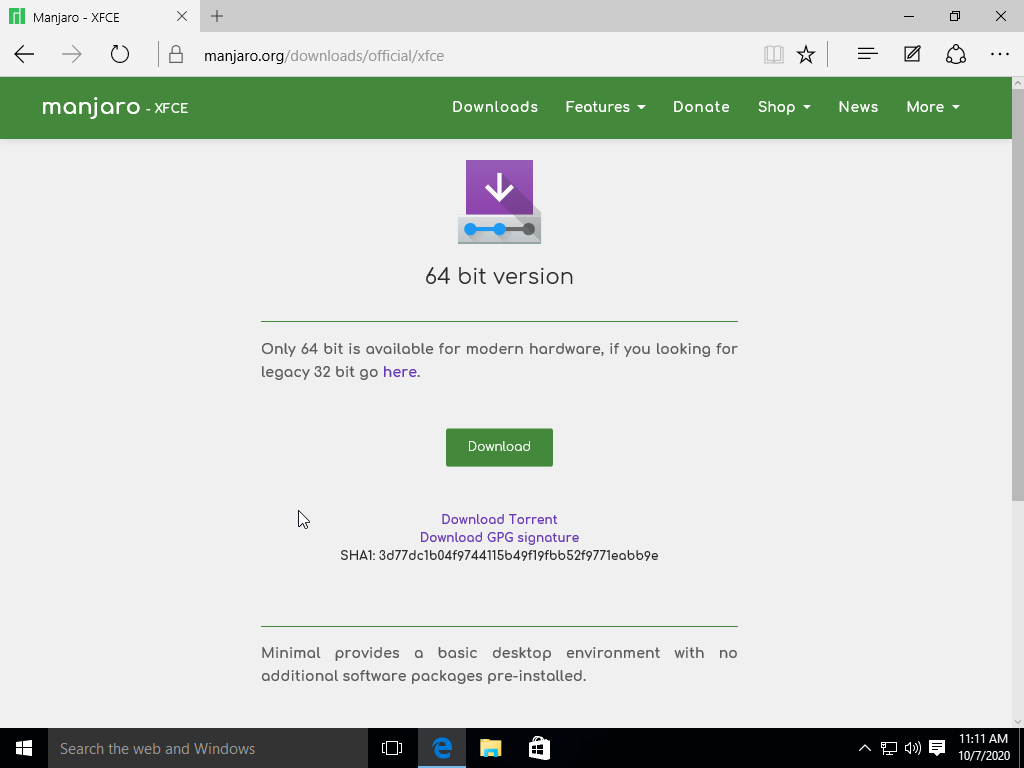
\includegraphics[width=.95\textwidth]{images/get_the_torrent_file.png}
        \caption{Manjaro XFCE download page.}%{ \url{https://manjaro.org/downloads/official/xfce/}}
        \label{fig:downloadPage}
    \end{minipage}\hfill
    \centering
    \begin{minipage}{0.5\textwidth}
        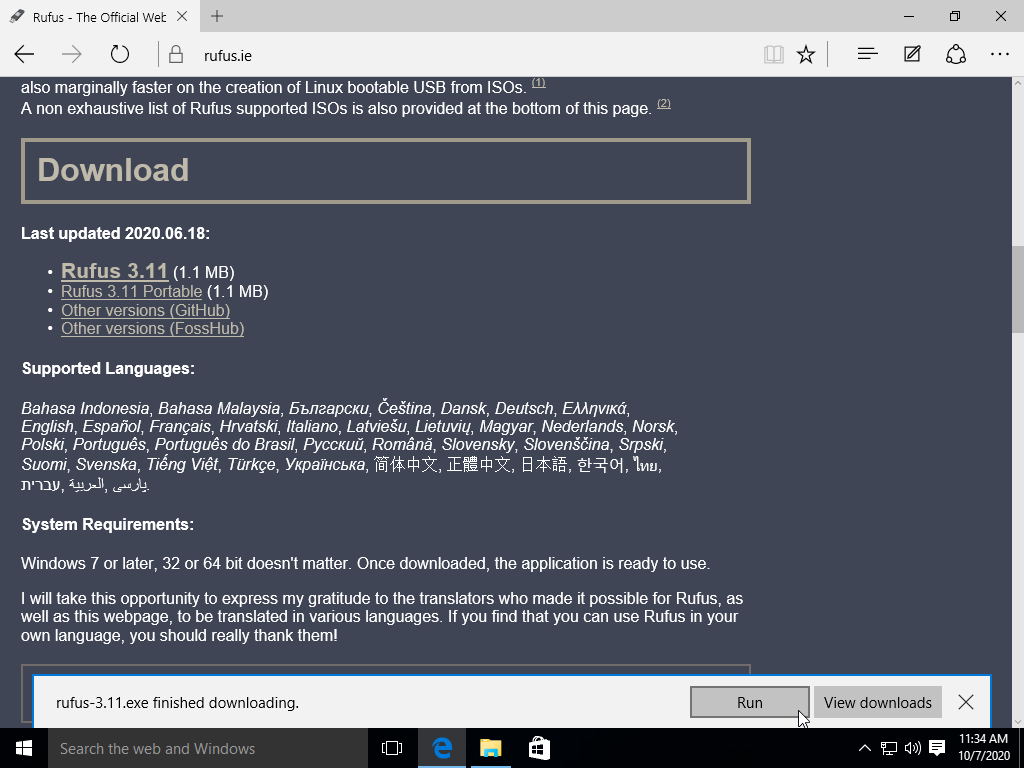
\includegraphics[width=.95\textwidth]{images/run_rufus.png}
        \caption{Download Rufus}%{ \url{https://manjaro.org/downloads/official/xfce/}}
        \label{fig:getRufus}
    \end{minipage}\hfill
    \centering
    \begin{minipage}{0.5\textwidth}
        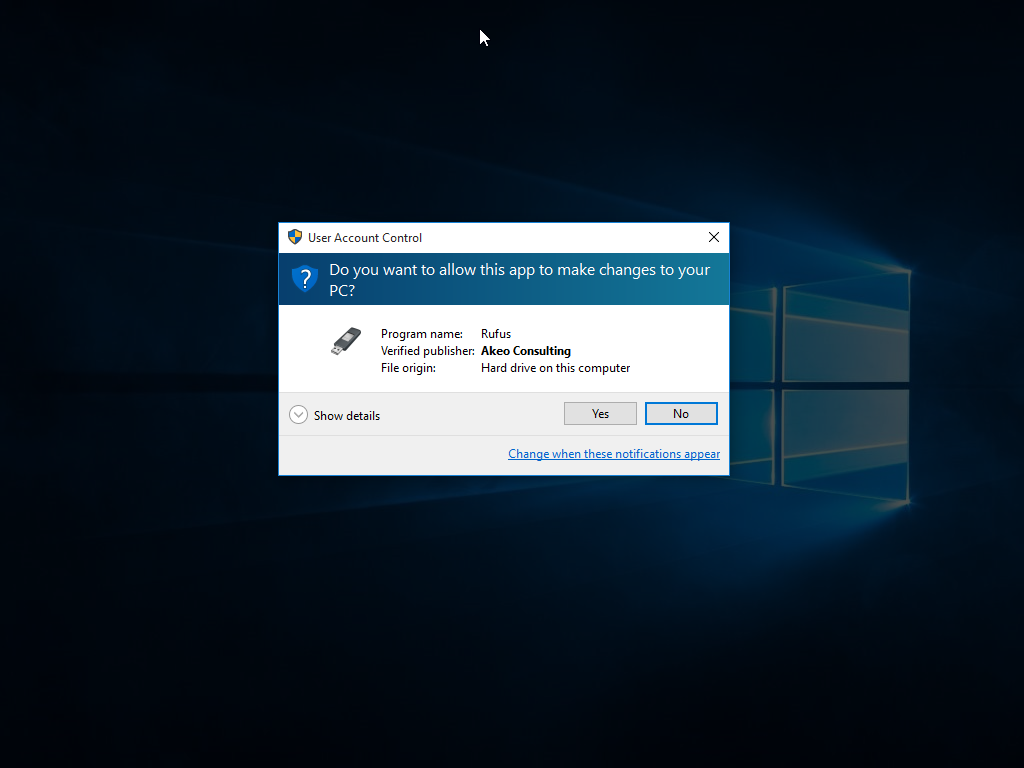
\includegraphics[width=.95\textwidth]{images/allow_rufus_to_run_if_asked.png}
        \caption{Run Rufus in Windows if asked}
        \label{fig:runRufus}
    \end{minipage}\hfill
    \centering
    \begin{minipage}{0.5\textwidth}
        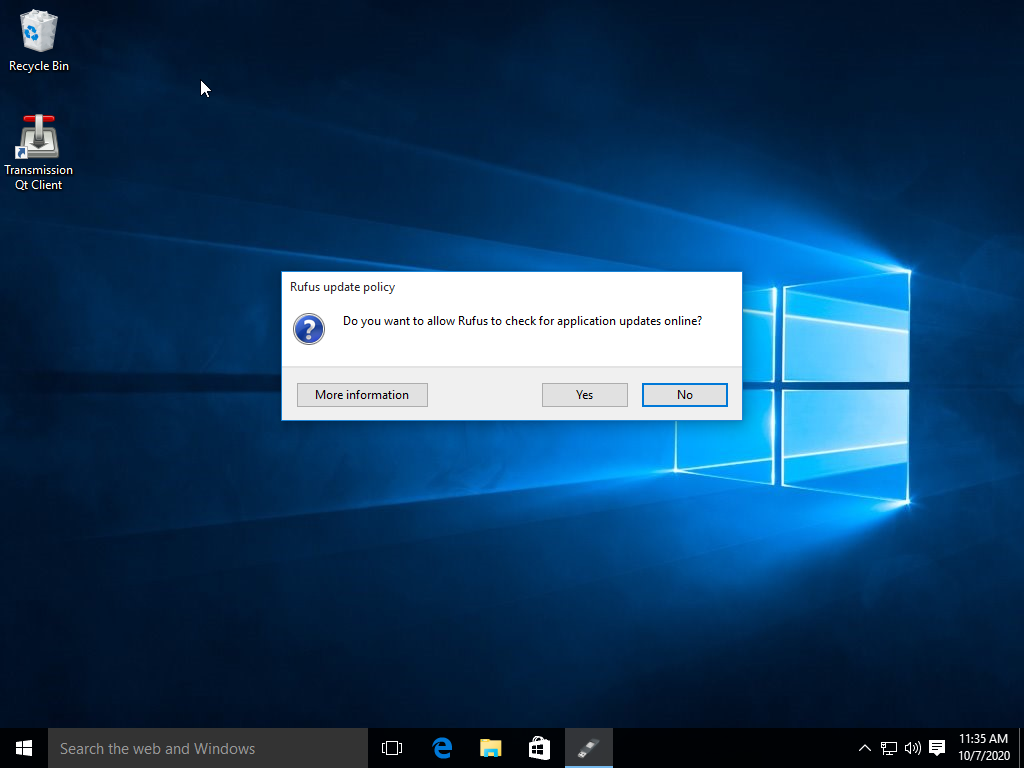
\includegraphics[width=.95\linewidth]{images/allow_rufus_to_check_for_updates_if_you_want.png}
        \caption{Update Rufus}
        \label{fig:updateRufus}
    \end{minipage}\hfill
    \centering
    \begin{minipage}{0.5\textwidth}
        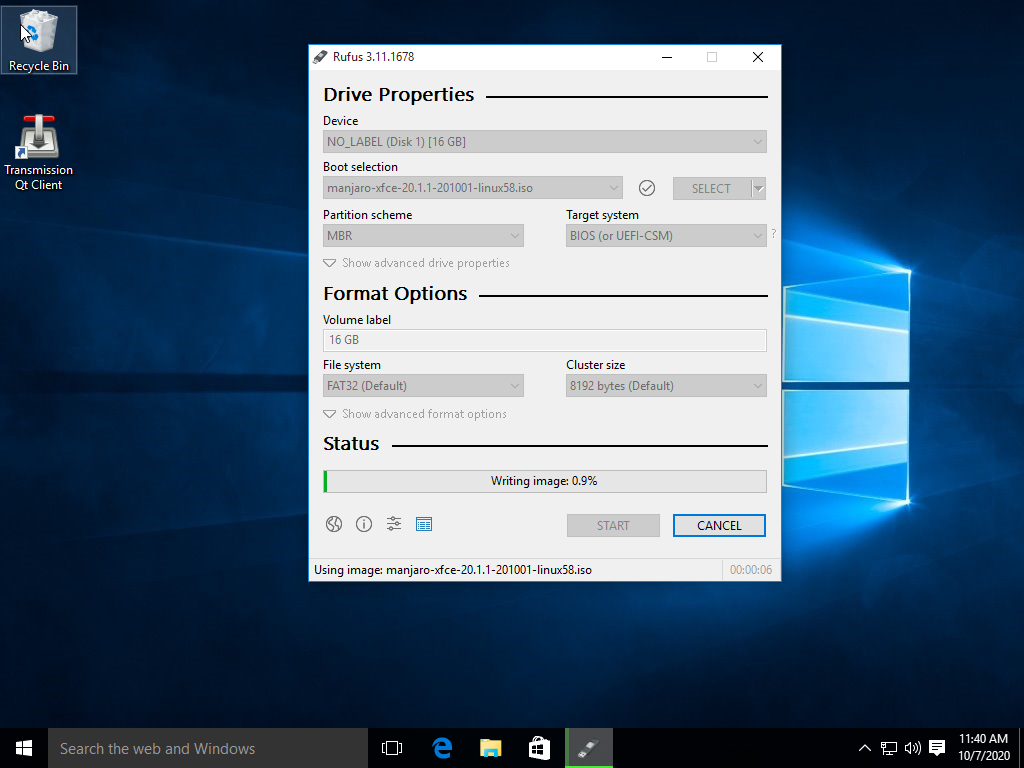
\includegraphics[width=.95\linewidth]{images/allow_some_time_for_rufus_to_install_the_iso_file_onto_the_flash_drive.png}
        \caption{See page \pageref{imageFile}, section \ref{imageFile}, items \ref{rufusBegin}-\ref{rufusEnd}}
        \label{fig:rufusInterface}
    \end{minipage}\hfill
    \centering
    \begin{minipage}{0.5\textwidth}
        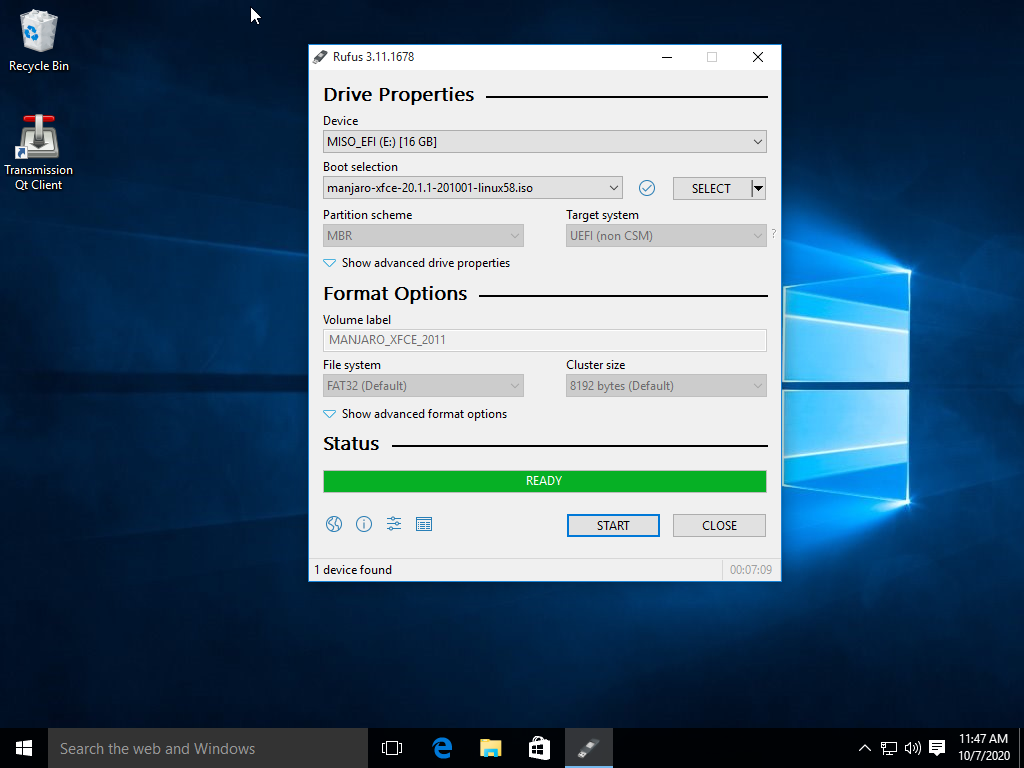
\includegraphics[width=.95\linewidth]{images/After_rufus_is_done_shutdown_youR_computer_and_say_good_buy_to_windows.png}
        \caption{Rufus once completed}
        \label{fig:rufusDone}
    \end{minipage}\hfill
\end{figure}

%%%%%%%%%%%%%LIVE BOOTING FIGURES SECTION%%%%%%%
\begin{figure}[ht!]
    \centering
    \begin{minipage}{0.5\textwidth}
        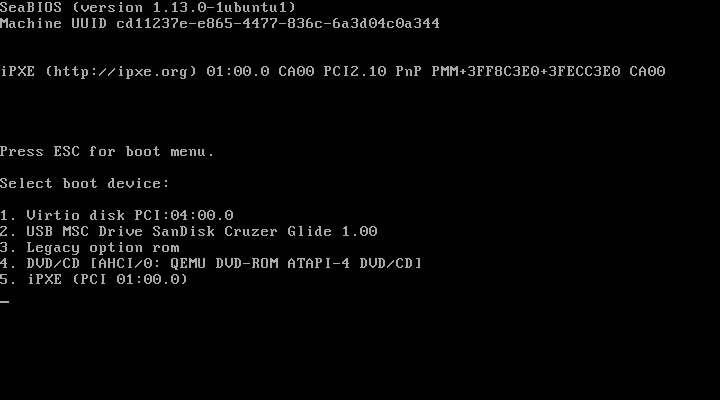
\includegraphics[width=.95\linewidth]{images/Boot_from_the_usb_this_is_different_on_all_devices.png}
        \caption{Boot into the flash drive}
        \label{fig:bootIntoFlash}
    \end{minipage}\hfill
    \centering
    \begin{minipage}{0.5\textwidth}
        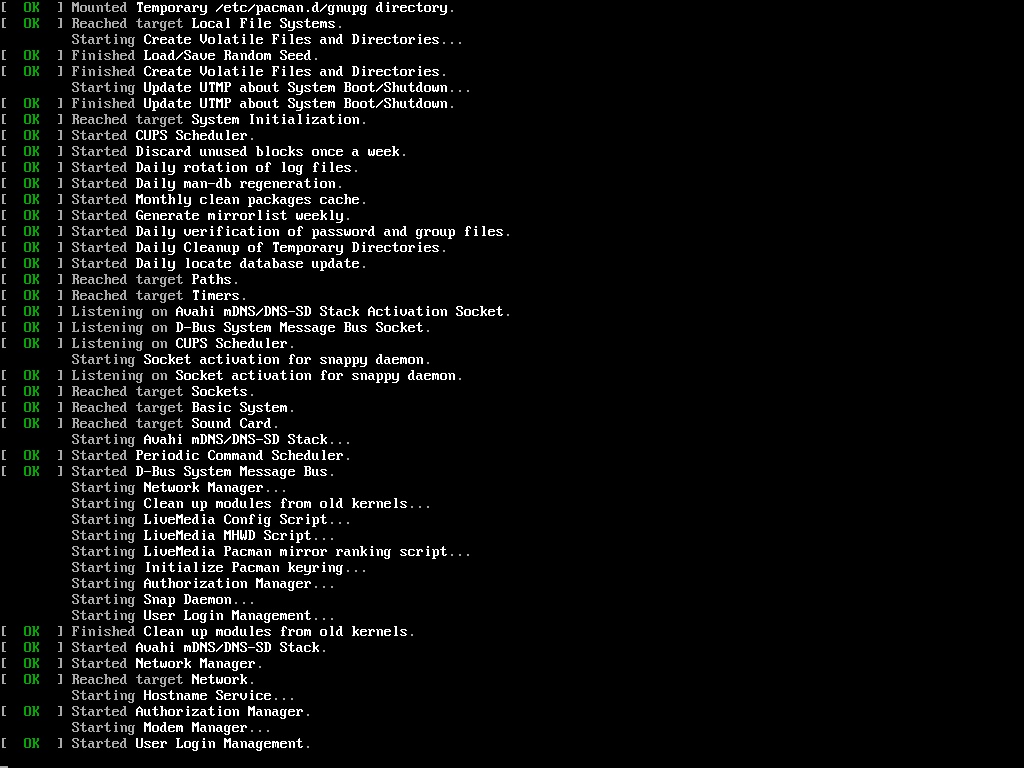
\includegraphics[width=.95\linewidth]{images/manjaro_will_flash_some_text_as_it_gets_setup.png}
        \caption{Normal first time boot sequence.}.
        \label{fig:bootSequence}
    \end{minipage}\hfill
    \centering
    \begin{minipage}{0.5\textwidth}
        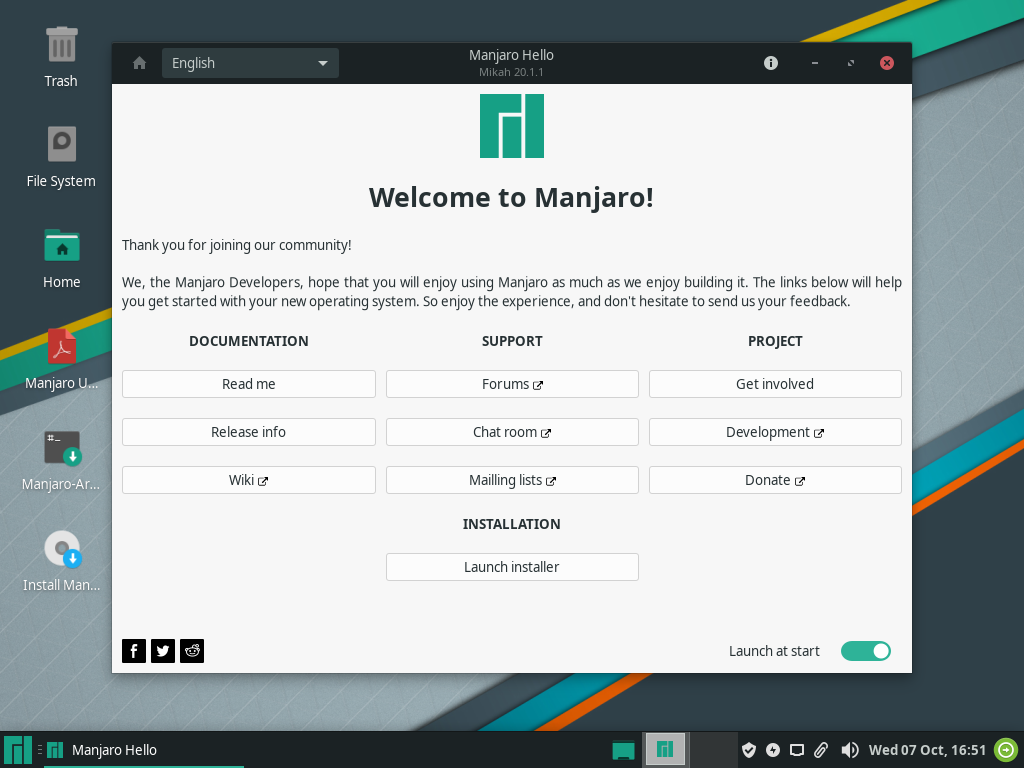
\includegraphics[width=.95\linewidth]{images/This_screen_means_you_can_explore_manjaro_before_you_destroy_windows.png}
        \caption{Manjaro first-time Welcome Screen}
        \label{fig:welcomeManjaro}
    \end{minipage}\hfill
\end{figure}

%%%%%%%%INSTALLATION FIGURES%%%%%%%%
\begin{figure}[ht!]
    \centering
    \begin{minipage}{0.5\textwidth}
        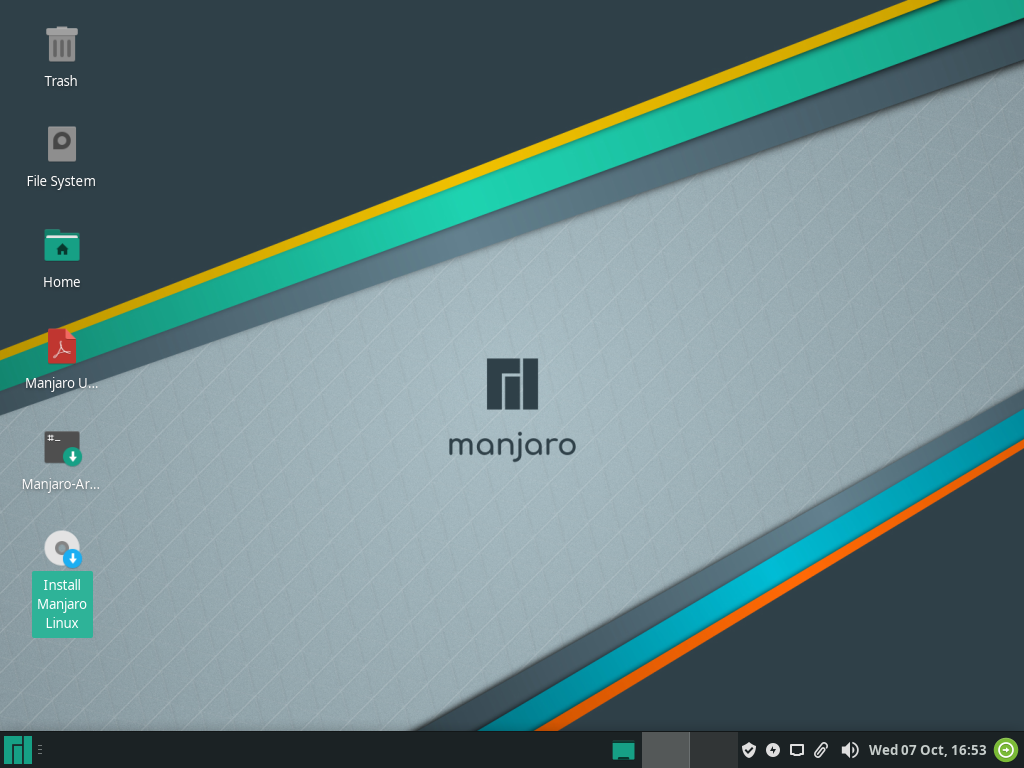
\includegraphics[width=.95\linewidth]{images/Once_ready_to_install_linux_choose_the_install_manjaro_button_from_the_home_screen.png}
        \caption{Find the ``Install'' button.}
        \label{fig:installManjaroButton}
    \end{minipage}\hfill
    \centering
    \begin{minipage}{0.5\textwidth}
        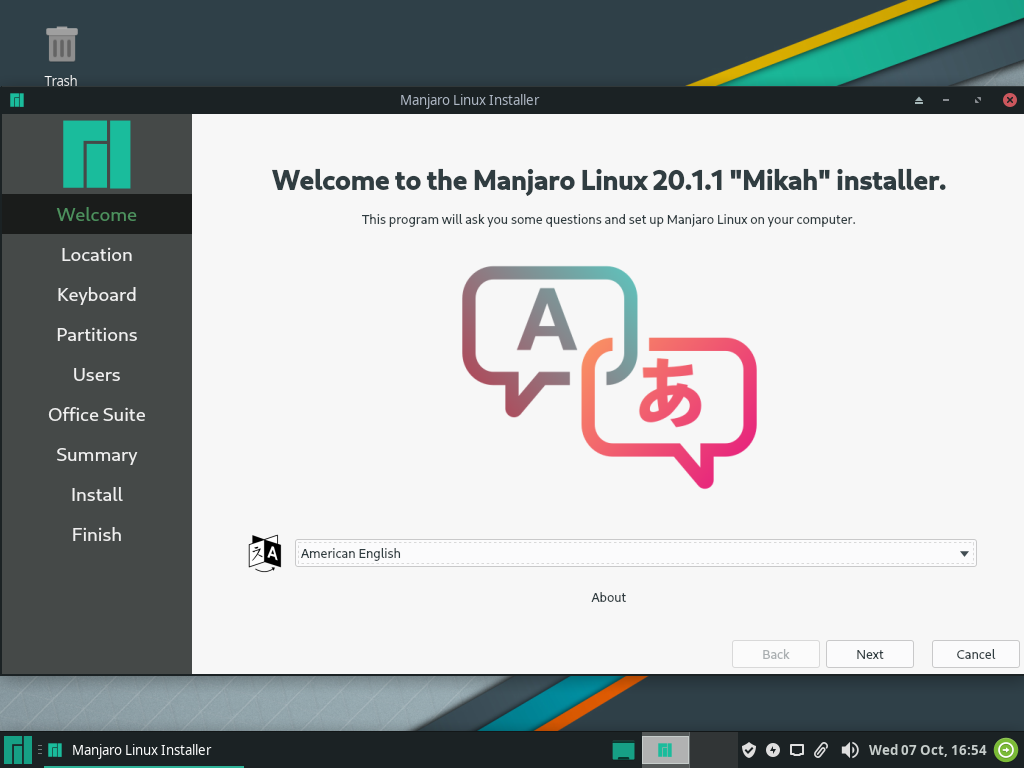
\includegraphics[width=.95\linewidth]{images/Choose_the_language_you_want_it_can_be_almost_any_language_and_linux_is_extremely_diverse.png}
        \caption{Choose your language.}
        \label{fig:chooseLanguage}
    \end{minipage}\hfill
    \centering
    \begin{minipage}{0.5\textwidth}
        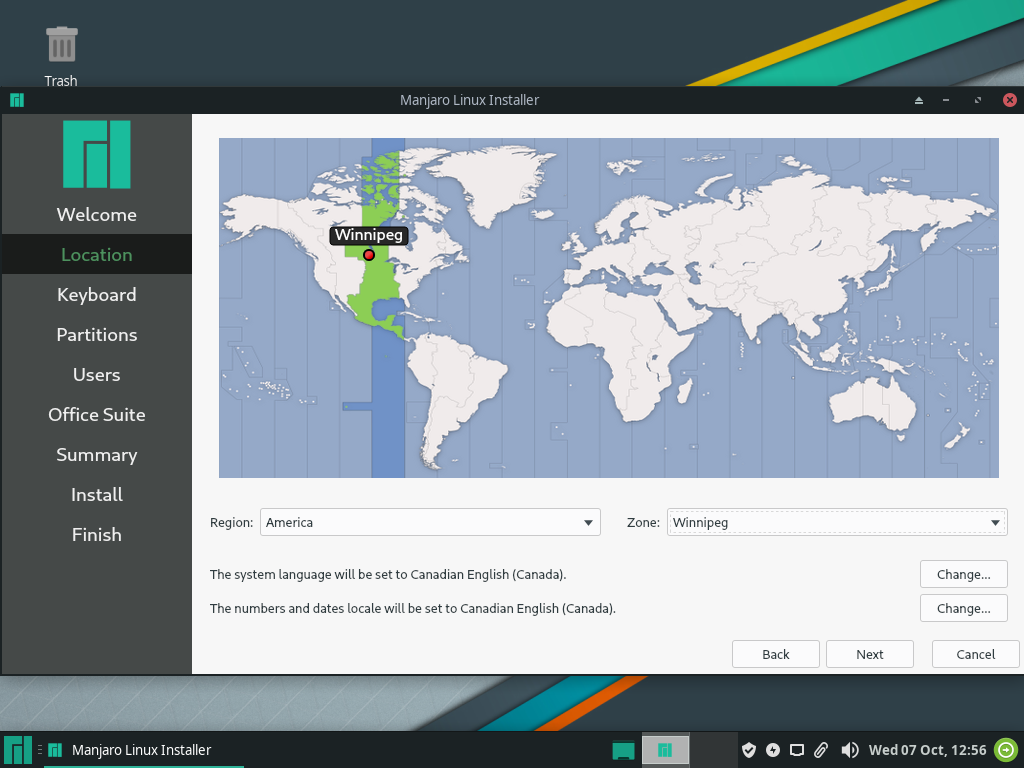
\includegraphics[width=.95\linewidth]{images/choose_your_time_zone_I_am_from_winnipeg_but_many_options_exist.png}
        \caption{Choose your time zone.}
        \label{fig:chooseTimeZone}
    \end{minipage}\hfill
    \centering
    \begin{minipage}{0.5\textwidth}
        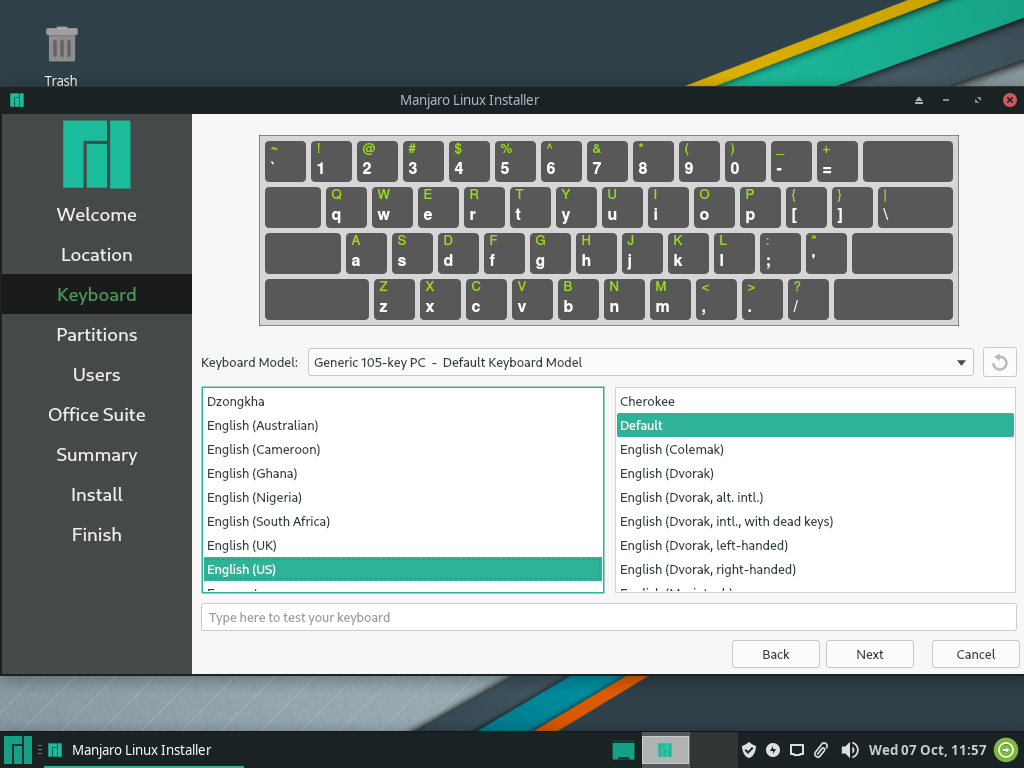
\includegraphics[width=.95\linewidth]{images/choose_your_keyboard_layout_most_people_have_the_default_but_it_should_be_able_to_be_customized_if_you_have_an_international_keyboard.png}
        \caption{Choose your keyboard.}
        \label{fig:chooseKeyboard}
    \end{minipage}\hfill
    \centering
    \begin{minipage}{0.5\textwidth}
        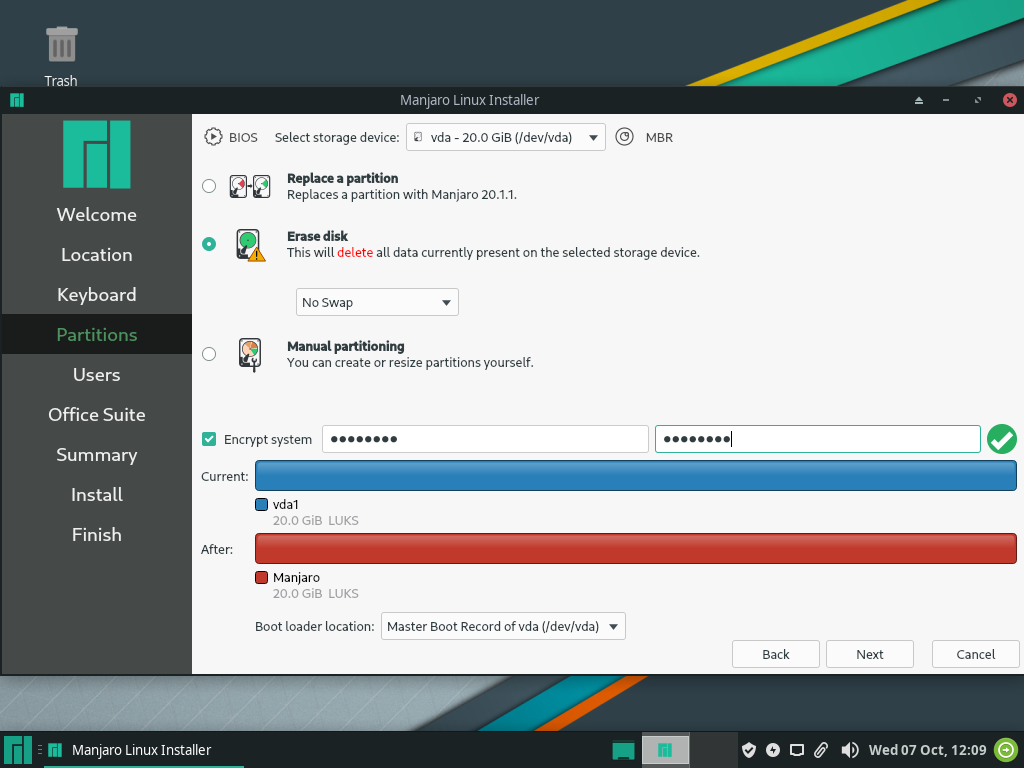
\includegraphics[width=.95\linewidth]{images/Choose_to_encrypt_your_system_to_avoid_any_snooping.png}
        \caption{See page \pageref{partitions} section \ref{install} item \ref{partitions}.}
        \label{fig:choosePartitioning}
    \end{minipage}\hfill
    \centering
    \begin{minipage}{0.5\textwidth}
        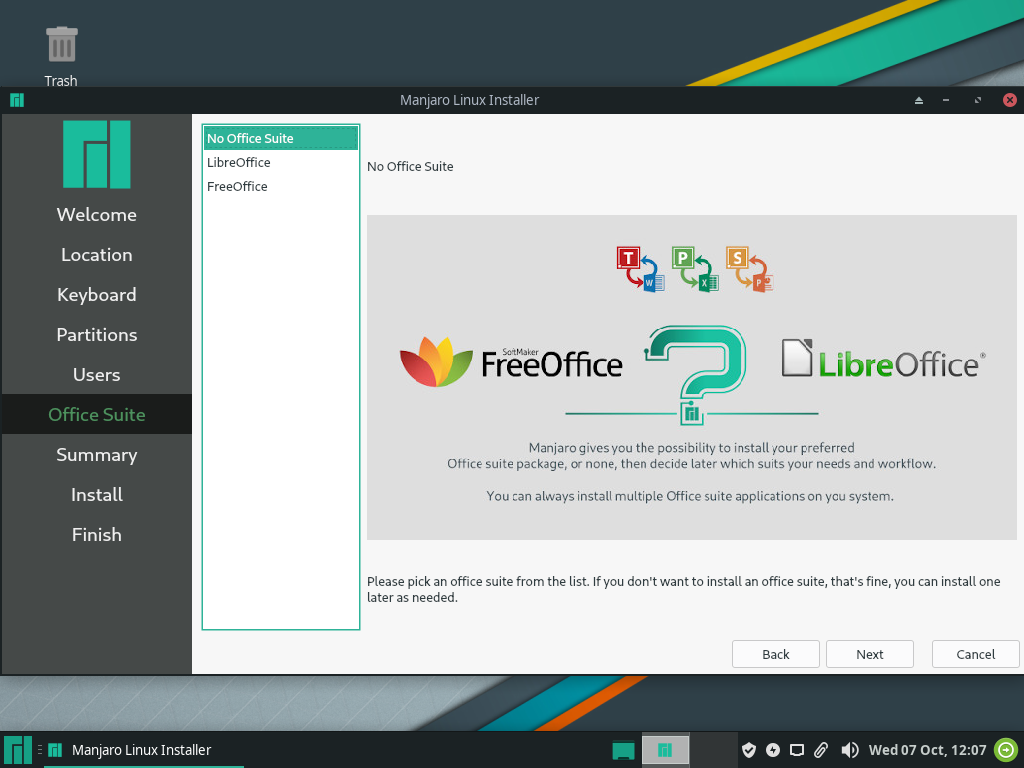
\includegraphics[width=.95\linewidth]{images/Choose_which_office_editor_you_want_if_any.png}
        \caption{Choose your office editor.}
        \label{fig:chooseOffice}
    \end{minipage}\hfill
\end{figure}

\begin{figure}[ht!]
    \centering
    \begin{minipage}{0.5\textwidth}
        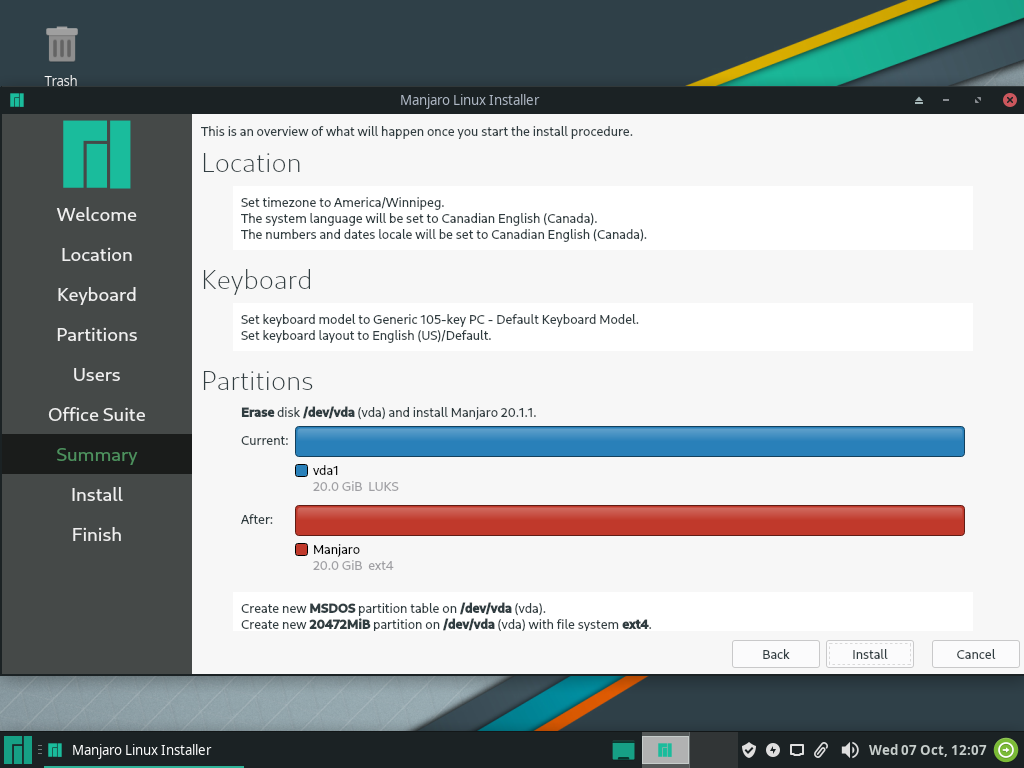
\includegraphics[width=.95\linewidth]{images/This_screen_is_a_summary_of_the_changes_you_want_to_make_make_sure_they_are_fine_as_after_this_step_linux_will_install.png}
        \caption{Manjaro install summary.}
        \label{fig:summaryPage}
    \end{minipage}\hfill
        \centering
    \begin{minipage}{0.5\textwidth}
        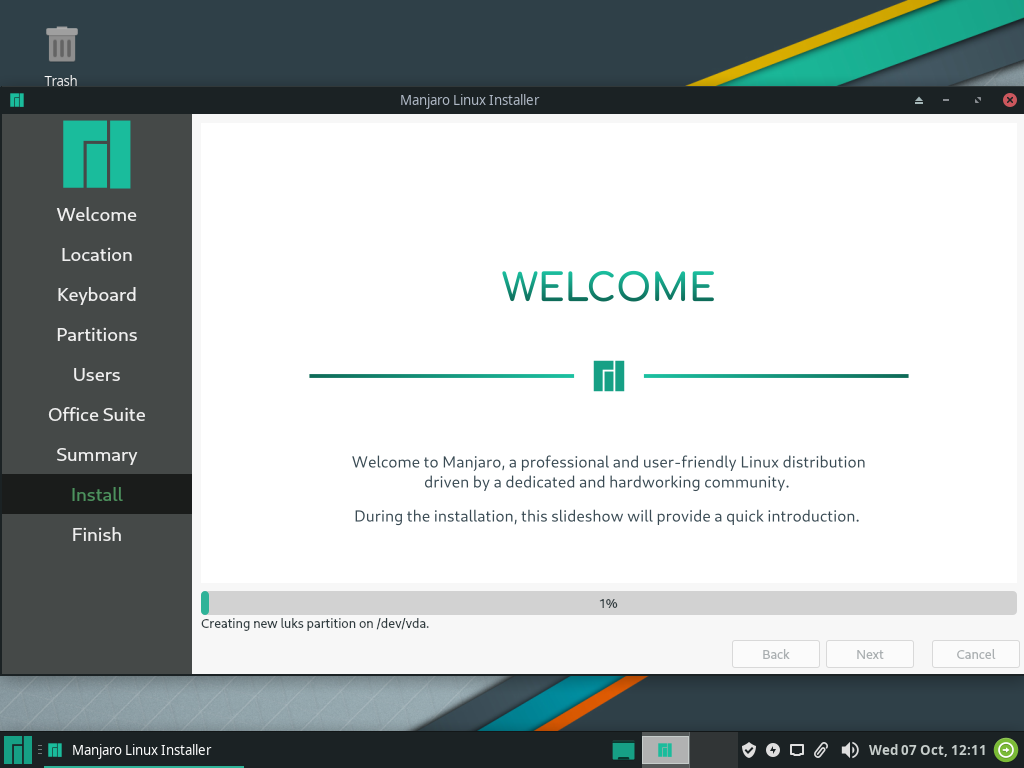
\includegraphics[width=.95\linewidth]{images/The_installation_will_take_a_while_especially_if_your_computer_is_slow_to_begin_with.png}
        \caption{Manjaro will now install.}
        \label{fig:actualInstallation}
    \end{minipage}\hfill
        \centering
    \begin{minipage}{0.5\textwidth}
        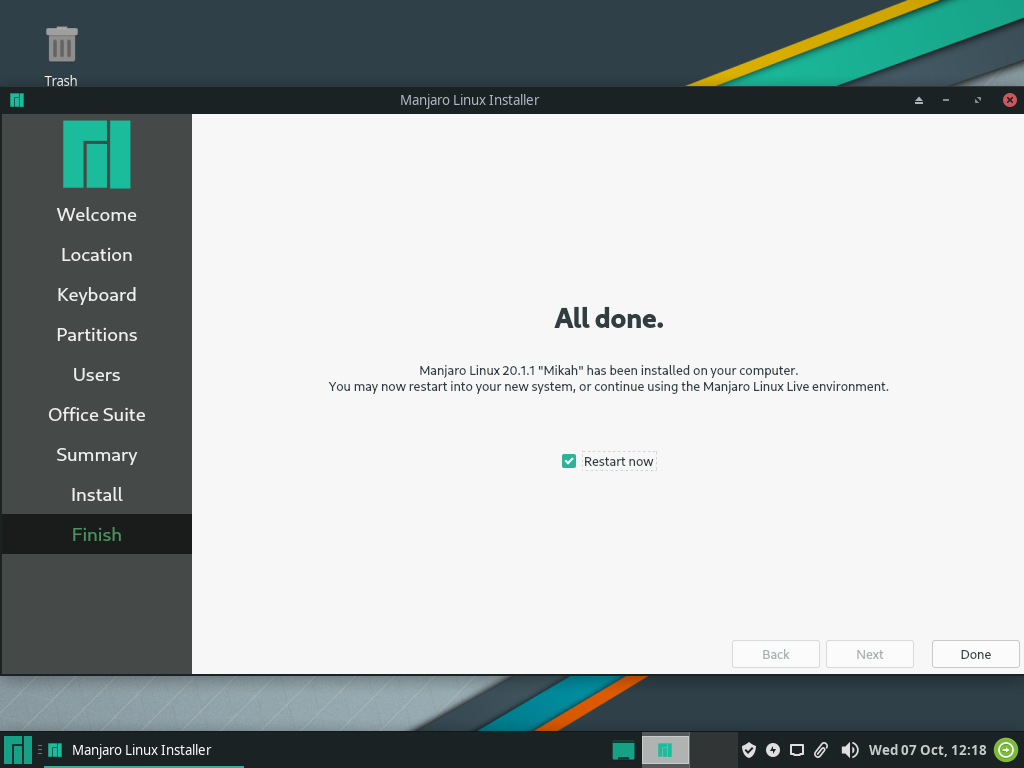
\includegraphics[width=.95\linewidth]{images/Restart_the_computer_to_first_login_to_the_installed_linux.png}
        \caption{Restart computer after installation}
        \label{fig:restartComputer}
    \end{minipage}\hfill
        \centering
    \begin{minipage}{0.5\textwidth}
        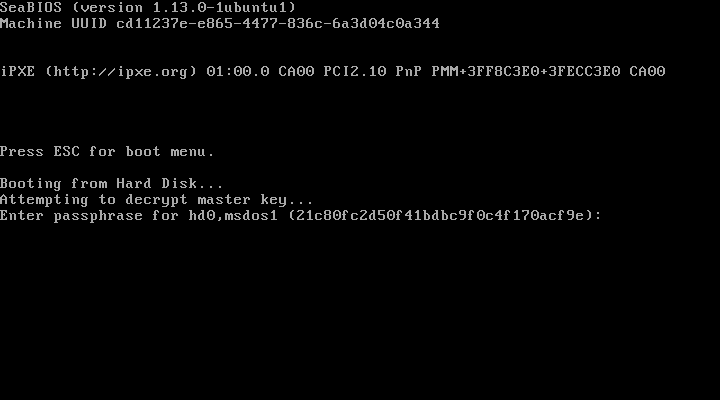
\includegraphics[width=.95\linewidth]{images/If_you_encrypted_the_file_system_you_will_be_asked_to_enter_the_encryptrion_key_every_time_you_turn_on_the_computer.png}
        \caption{Decrypt the computer if you encrypted it.}
        \label{fig:decryptComputer}
    \end{minipage}\hfill
        \centering
    \begin{minipage}{0.5\textwidth}
        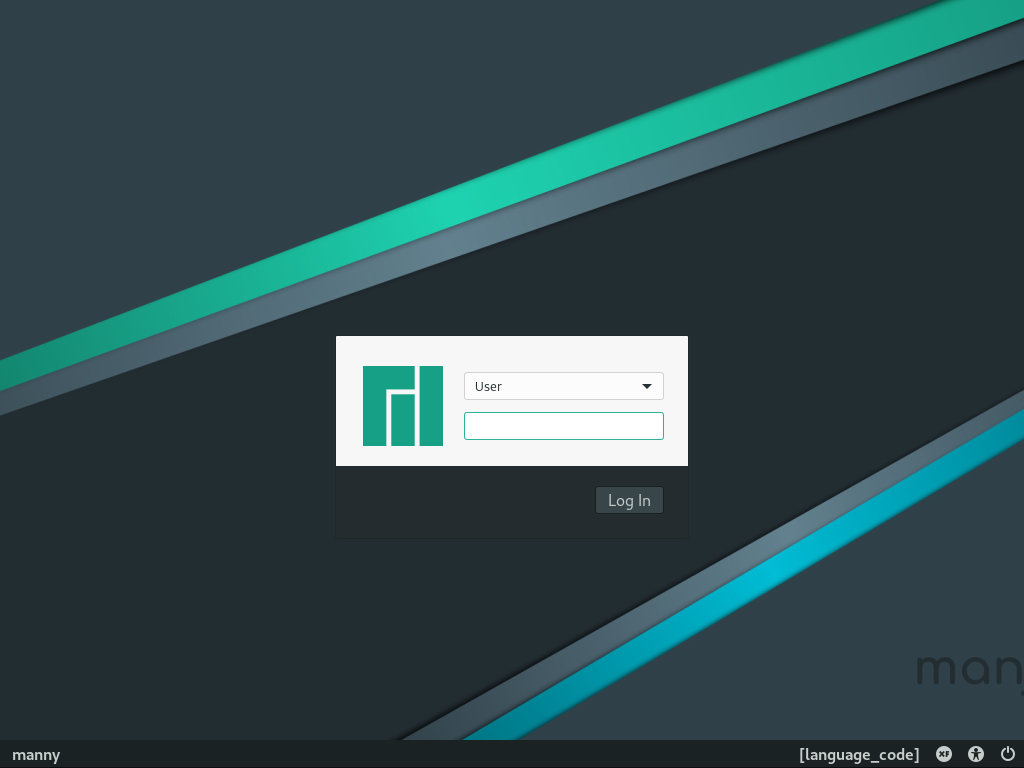
\includegraphics[width=.95\linewidth]{images/Login_for_the_first_time.png}
        \caption{Login for the first time.}
        \label{fig:loginPage}
    \end{minipage}\hfill
        \centering
    \begin{minipage}{0.5\textwidth}
        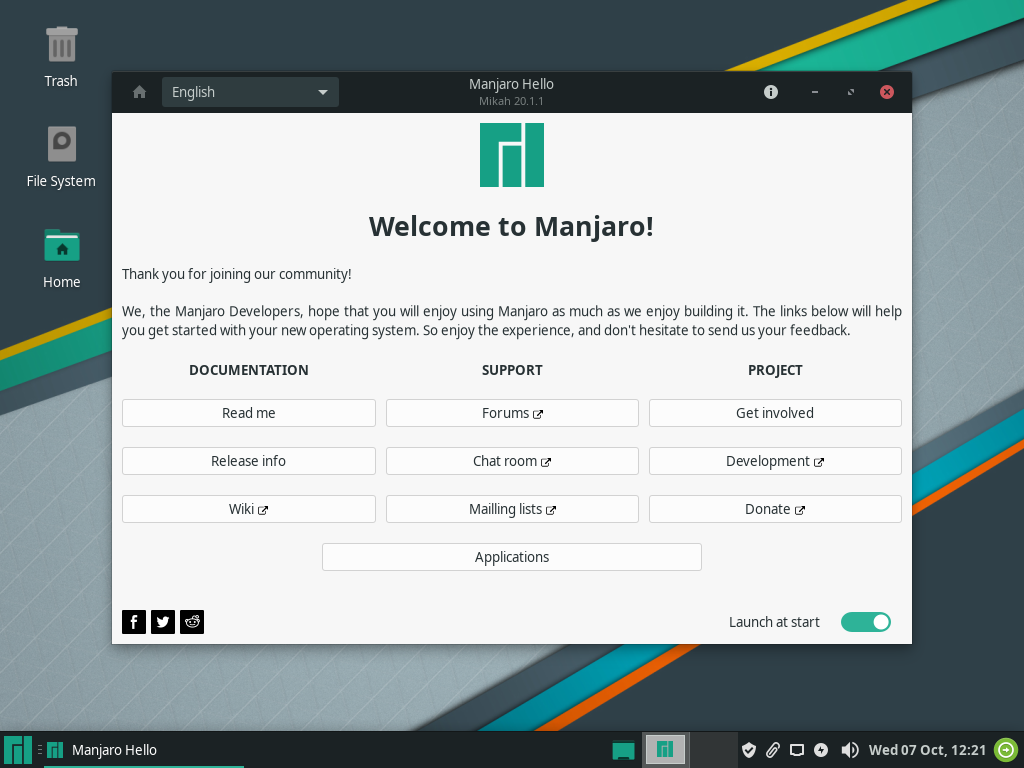
\includegraphics[width=.95\linewidth]{images/Now_you_have_linux_installed.png}
        \caption{Manjaro is now installed, have fun.}
        \label{fig:finalPage}
    \end{minipage}\hfill
    
\end{figure}


\end{document}
